\chapter{Applicazione}
\label{chapter:app}
Un ulteriore aspetto chiave del progetto è l'applicazione Android. 
Si posiziona in un livello di mezzo tra l'utente e il classificatore.

Attraverso l'uso dei sensori inerziali del dispositivo è possibile richiedere al sistema di ipotizzare l'attività che si sta svolgendo 
oppure addestrare lo stesso sistema con una precisa attività tra quelle selezionabili.




\subsubsection{Compatibilità}
Si offre una compatibilità con tutte le versioni di Android che supportano almeno la versione delle API 16, nella pratica tutte
le versioni maggiori o uguali ad Android 4.1 rilasciato nel 2012. 

Al momento della stesura di questa relazione corrisponde ad assicurare il funzionamento dell'app sul 99,8\% dei dispositivi 
con questo sistema operativo.

\subsubsection{Internazionalizzazione}
L'intero applicativo è dotato di supporto multilingua: italiano e inglese.

\subsubsection{Linguaggi di sviluppo}
I linguaggi utilizzati sono stati: 
\begin{itemize}
    \item \textit{Java} per lo sviluppo dei processi software
    \item \textit{XML} per tutti i layout
\end{itemize}


\newpage
\section{Interfaccia}
L'applicazione presenta un'interfaccia minimale sviluppata secondo le linee guida dell'ormai noto Material Design.

\subsubsection{Material Design}
Con Material Design \cite{material} si intende un linguaggio visivo che sintetizza i principi classici 
del buon design utilizzando le nuove innovazioni della tecnologia e della scienza.

L'intero linguaggio si basa sul concetto fisico di "Materiale" di cui si vuole effettuare una trasposizione nel 
design di tutte le caratteristiche (luci, ombre, etc.) che lo definiscono nel mondo reale.

\subsubsection{Suddivisione per funzionalità}
La suddivisione delle sezioni dell'applicazione segue perfettamente le funzionalità da essa offerte: 
l'analisi dell'attività, l'apprendimento di una attività e l'inserimento di informazioni aggiuntive.
\begin{figure}[H]
    \centering
    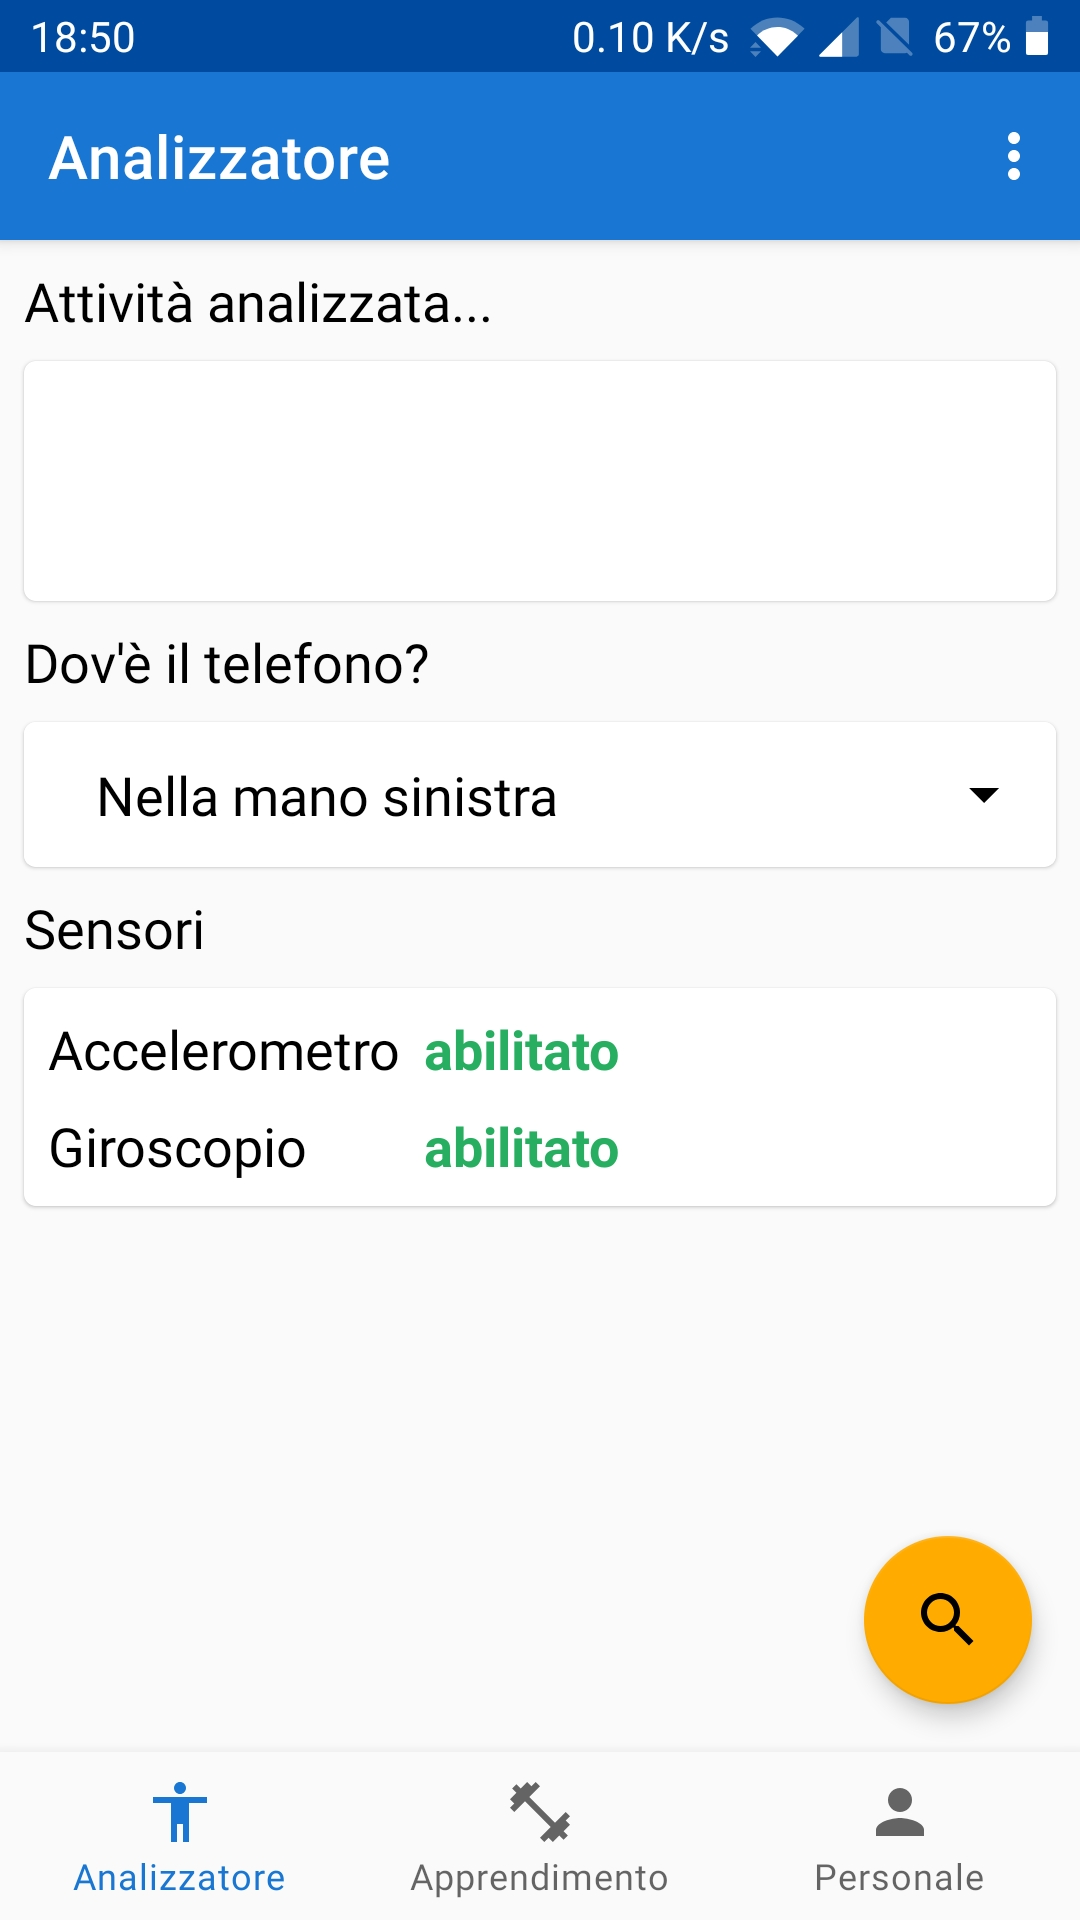
\includegraphics[scale = 0.1019]{assets/images/screenshots/1a_Init.jpg}
    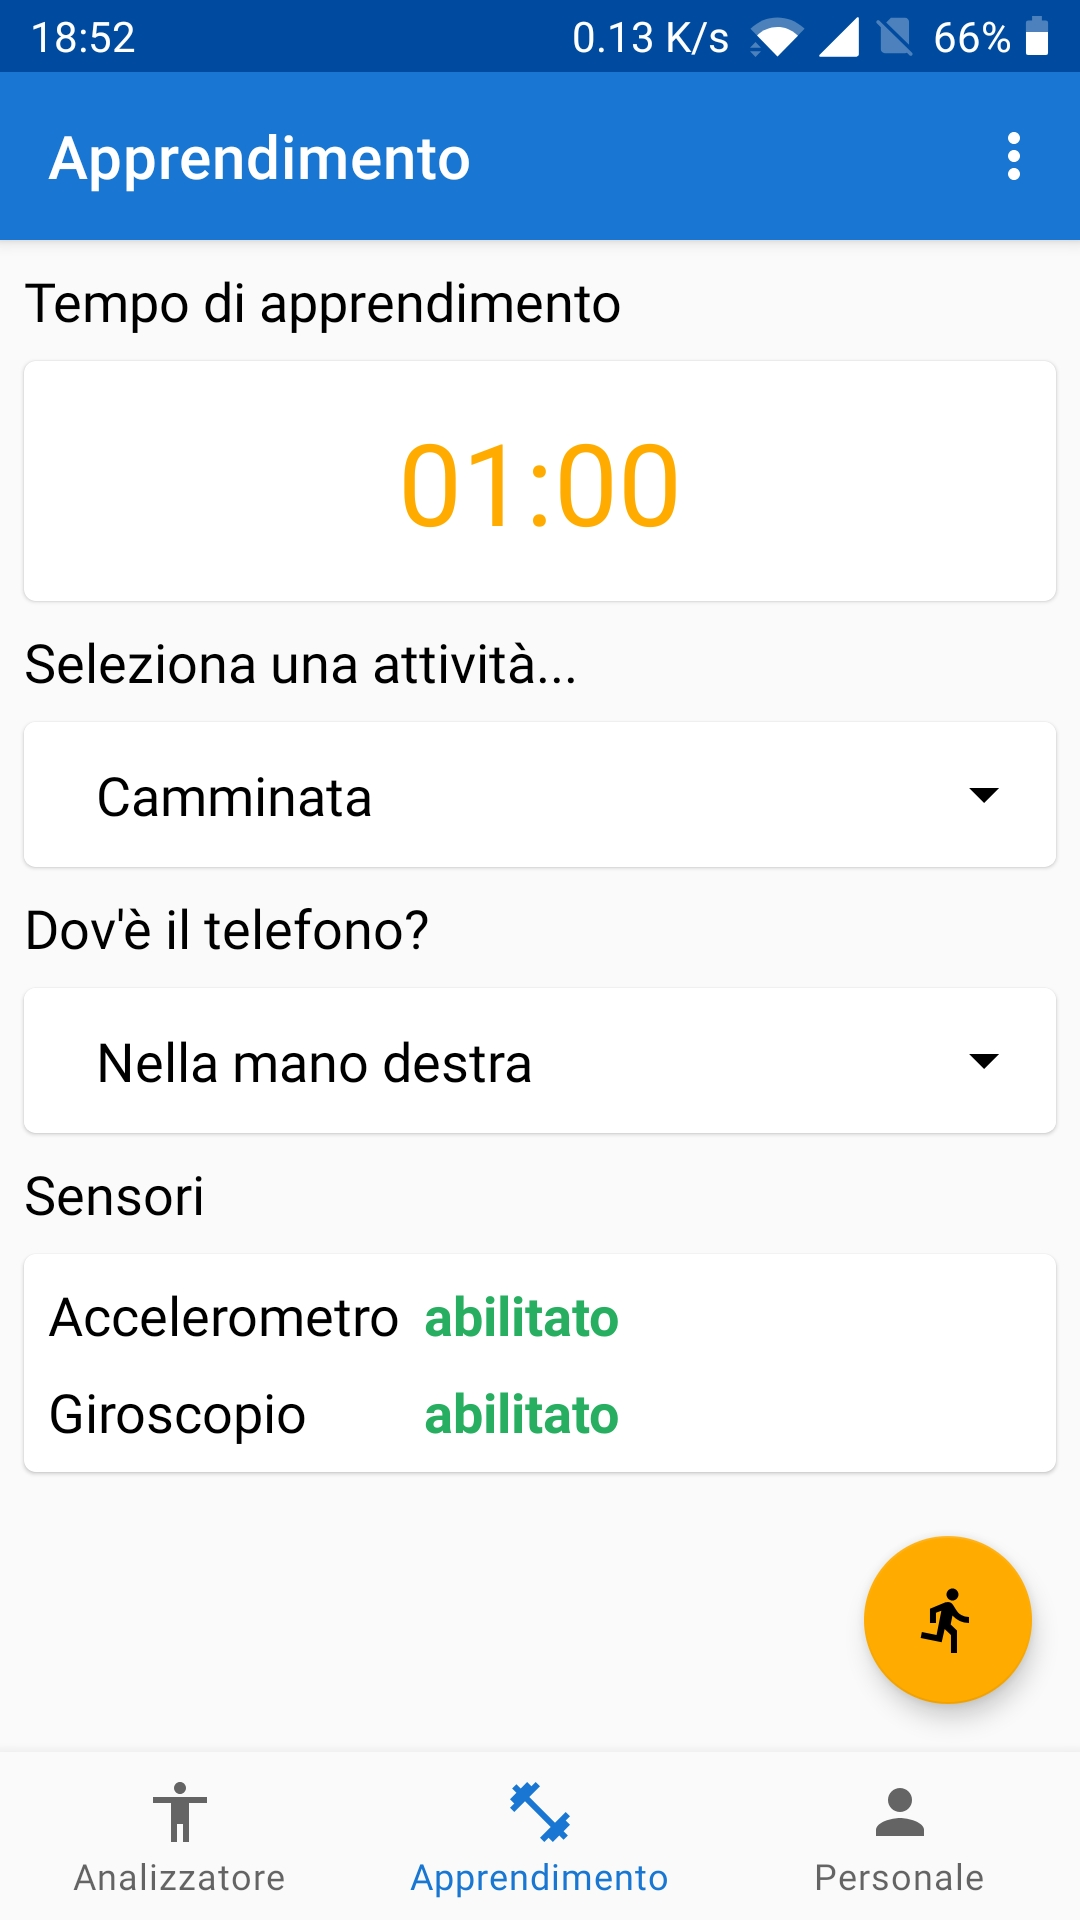
\includegraphics[scale = 0.1019]{assets/images/screenshots/2a_Init.jpg}
    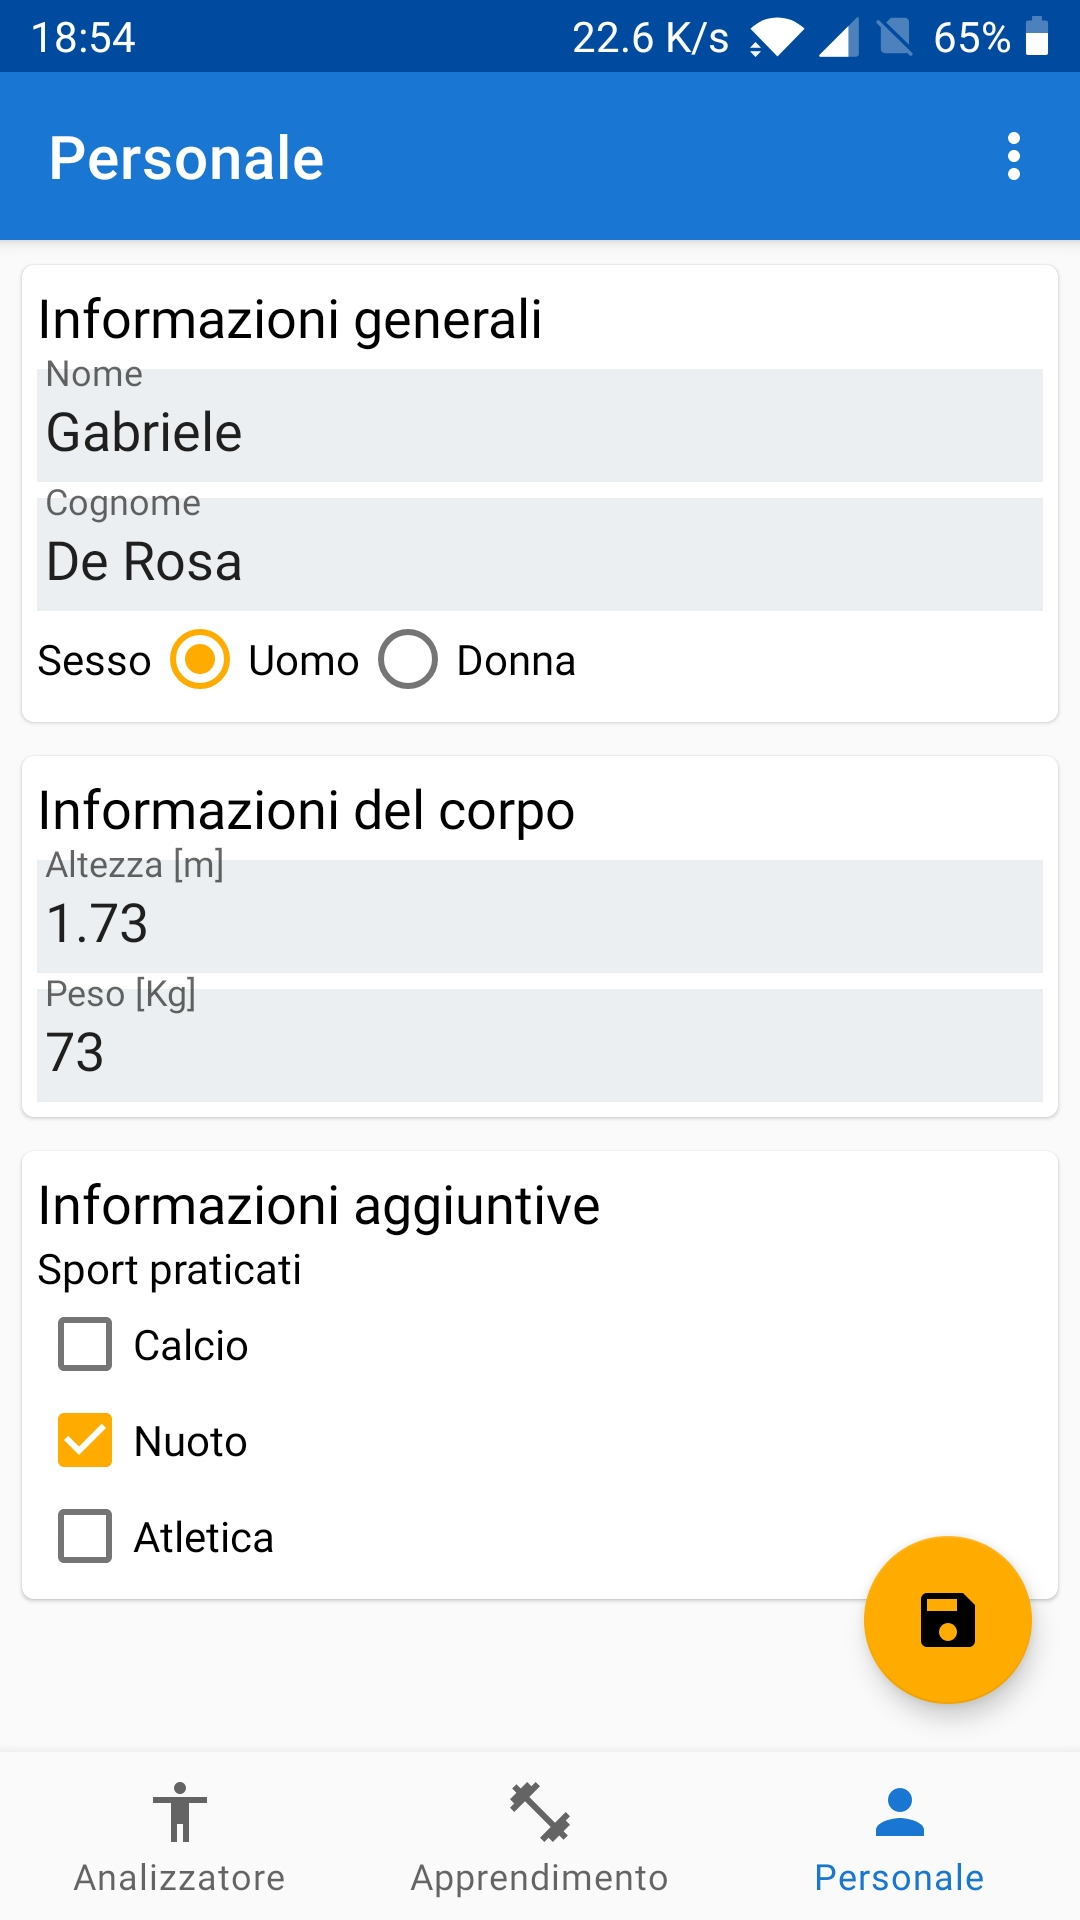
\includegraphics[scale = 0.1019]{assets/images/screenshots/3a_Init.jpg}
    \caption{Le 3 sezioni principali dell'applicazione}
    \label{fig:screenshots}
\end{figure}


\subsection{Sezione di analisi}
La sezione di analisi consente di testare l'efficacia del classificatore. 
Si vuole ottenere in risposta un riscontro sull'attività che si sta svolgendo.

La raccolta dei dati inerziali procede con l'invio delle informazioni al server che, 
come abbiamo visto nella sezione \ref{section:receiver}, dopo l'elaborazione restituirà in risposta l'ipotesi.


\subsubsection{Fase 1: Inizializzazione}
In una prima fase l'applicazione richiede in autonomia alle API le informazioni relative alle posizioni del dispositivo 
che sono disponibili.

Dopo aver ottenuto una risposta simile a quella mostrata nel codice \ref{listing:response-positions}  
l'utente ha la possibilità di selezionare la posizione, tra quelle scaricate, in cui desidera tenere 
il dispositivo durante l'esecuzione dell'attività. In seguito a questa scelta l'analisi può essere avviata.

\subsubsection{Fase 2: Preparazione}
All'avvio dell'analisi sarà inizializzato un servizio in foreground \cite{services} che si occuperà di svolgere tutte le azioni 
necessarie per le fasi seguenti. La UI continuerà ad essere aggiornata con le informazioni ricevute dal servizio.

Il primo obiettivo è quello di contattare il server per stabilire una connessione TCP ed iniziare lo scambio dati. 
Qualora la connessione avvenisse con successo passerà qualche altro secondo prima che i sensori inizino la raccolta dei dati.
Questo \textit{tempo di preparazione} è pensato appositamente in modo da consentire all'utente 
di prepararsi posizionando il dispositivo nella posizione selezionata. Nella UI è mostrato un countdown.

\subsubsection{Fase 3: Analisi}
Allo scadere del conto alla rovescia i sensori sono abilitati. 
Ogni informazione raccolta è inserita in un messaggio simile a quello visto 
nell'esempio \ref{listing:example-message-learning} e subito inviata.

\subsubsection{Fase 4: Predizione}
Durante la fase di analisi, e ininterrottamente fino allo stop dell'utente, il processo resta in ascolto, in attesa di 
messaggi di risposta dal server.
La maggioranza delle risposte sono messaggi di conferma di avvenuta ricezione delle informazioni e messaggi contenenti 
le ipotesi stipulate dal classificatore sull'attività in corso di esecuzione.
In questa seconda eventualità i risultati vengono mostrati all'utente.
\begin{figure}[H]
    \centering
    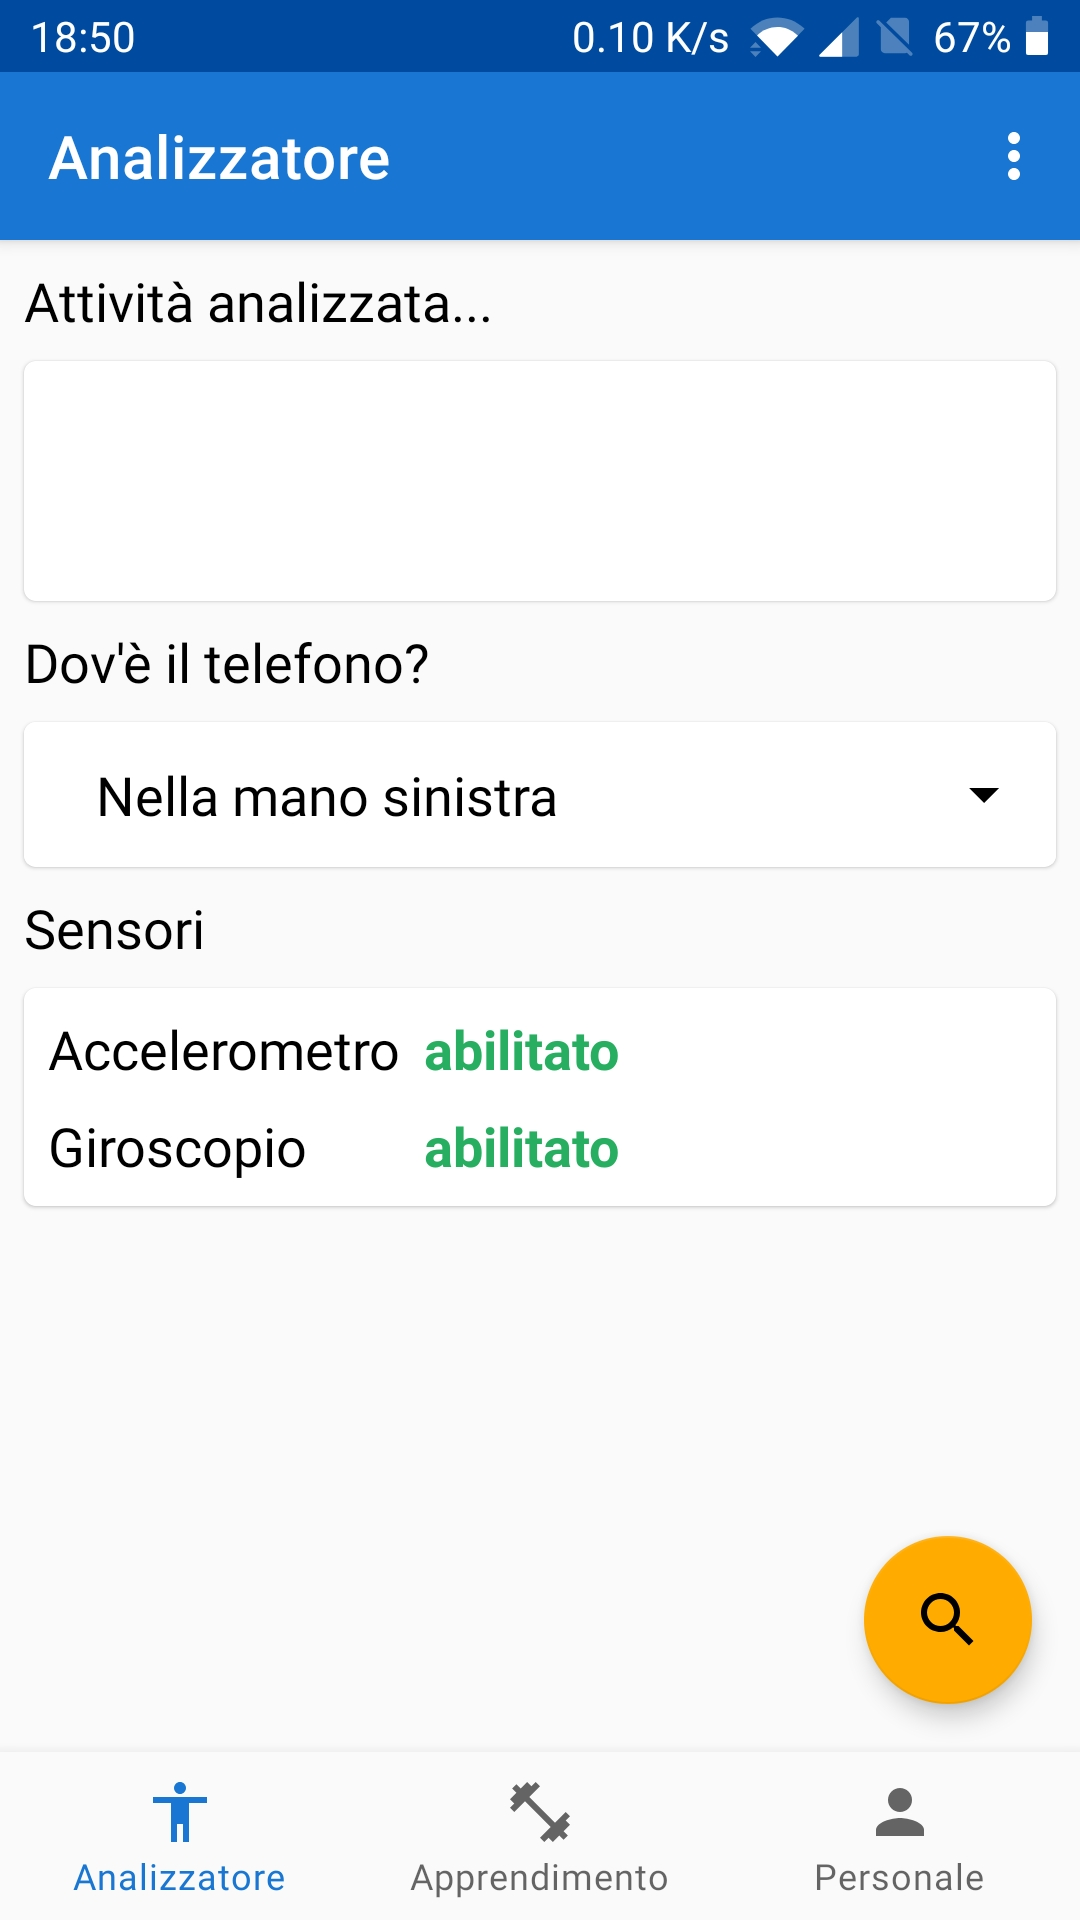
\includegraphics[scale = 0.1019]{assets/images/screenshots/1a_Init.jpg}
    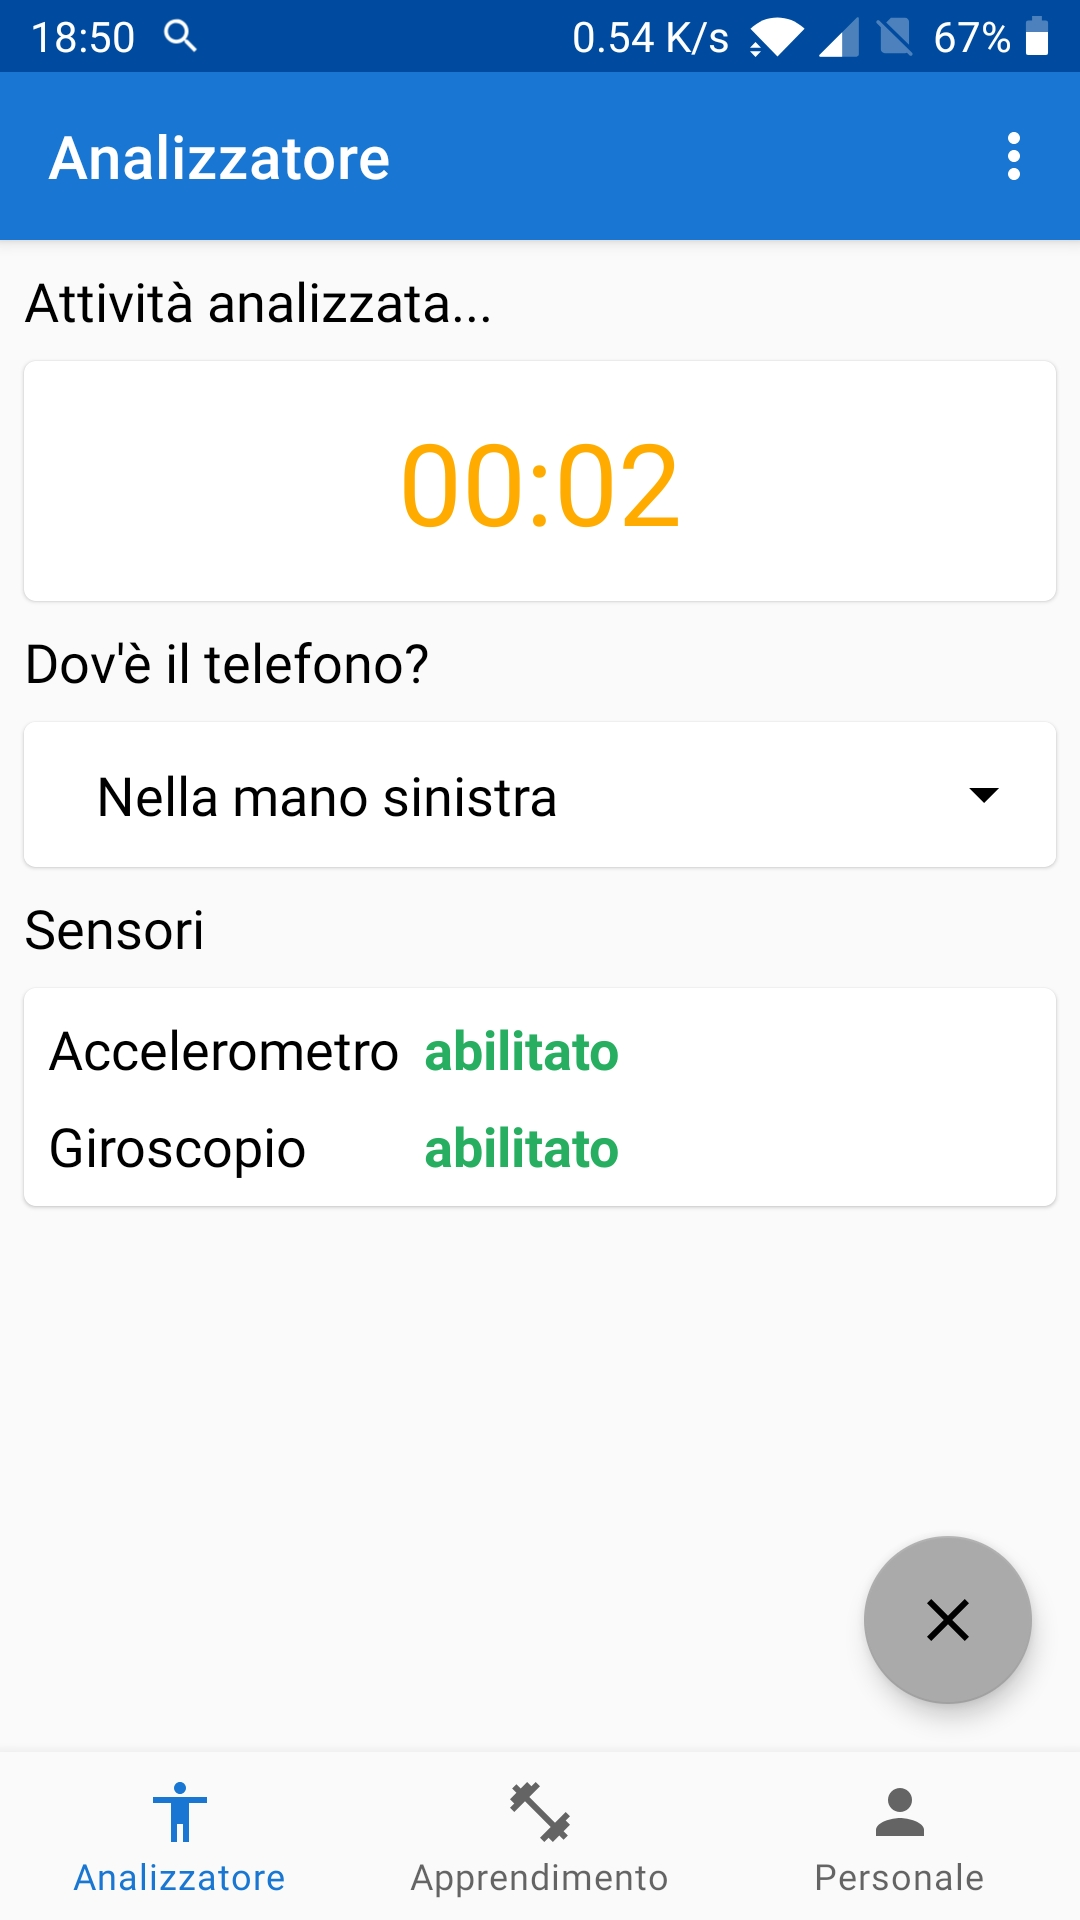
\includegraphics[scale = 0.1019]{assets/images/screenshots/1b_Preparation.jpg}
    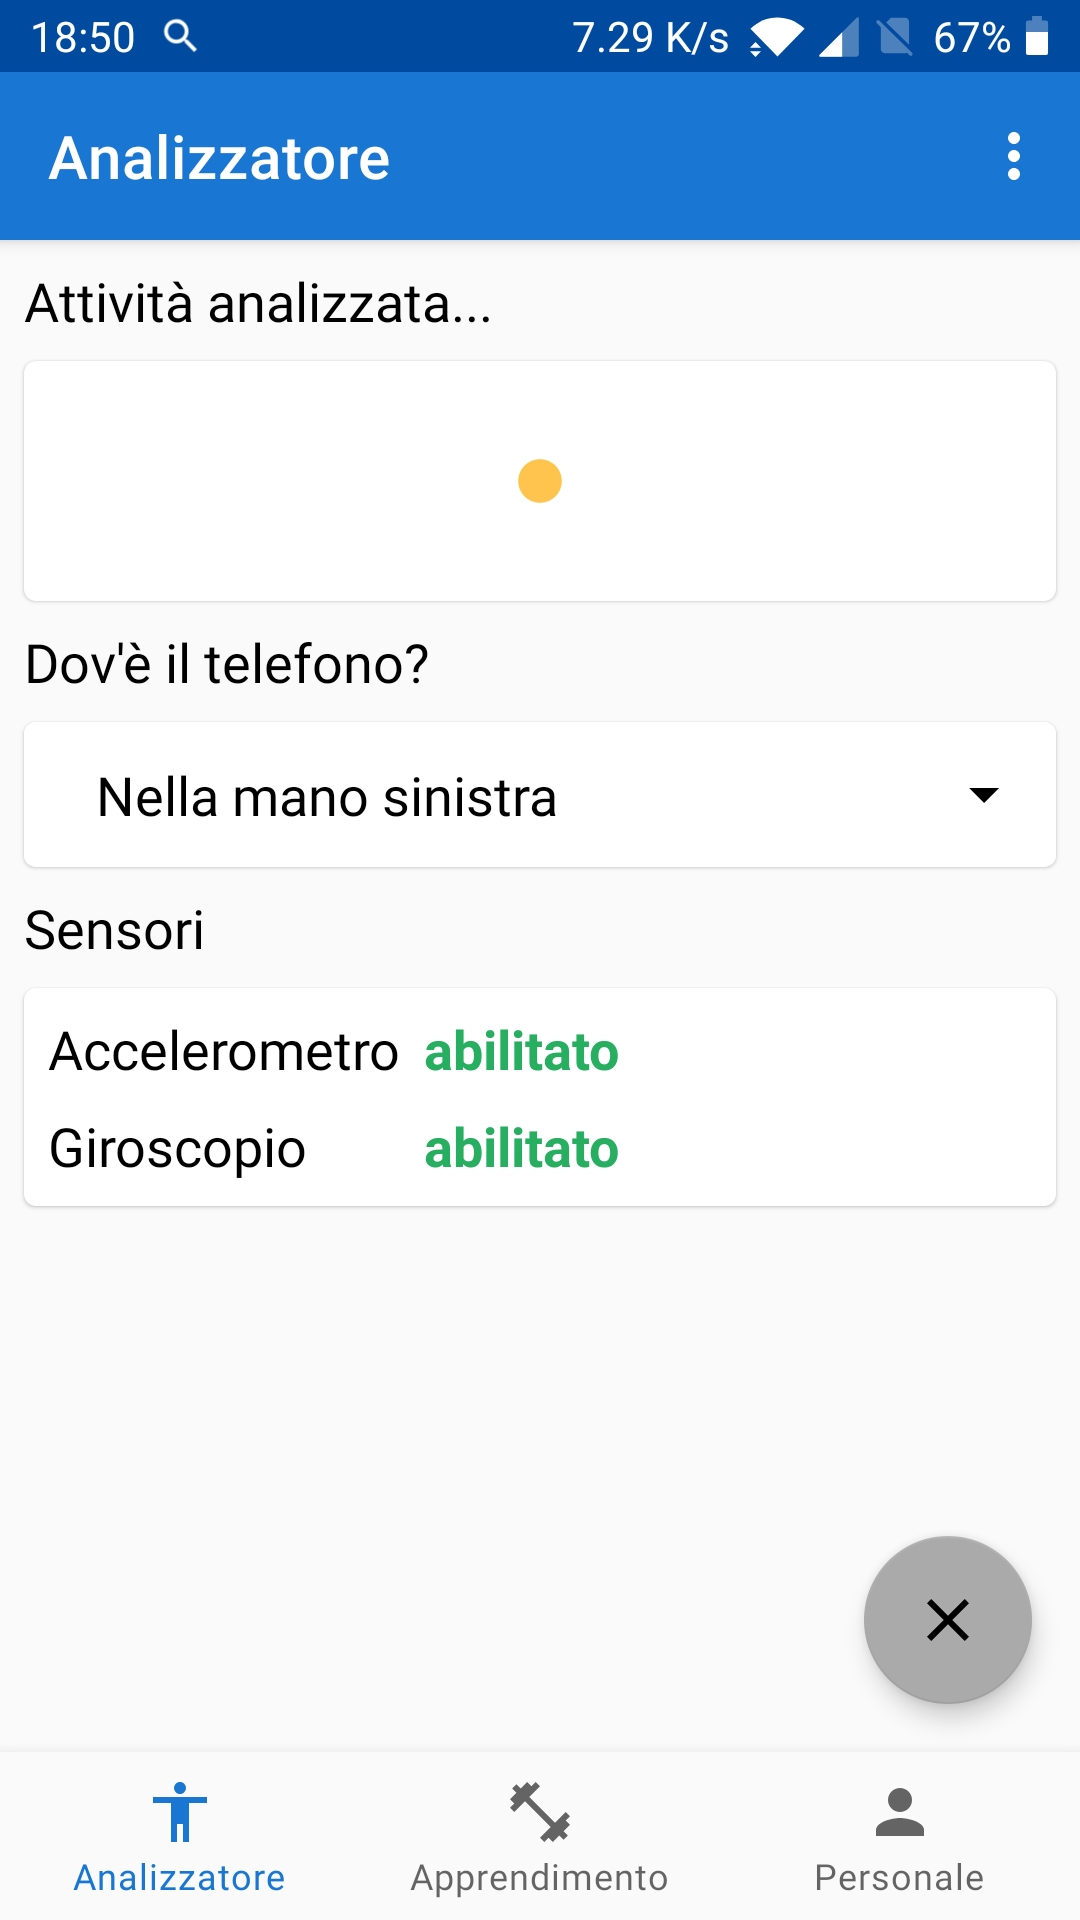
\includegraphics[scale = 0.1019]{assets/images/screenshots/1c_Analysis.jpg}
    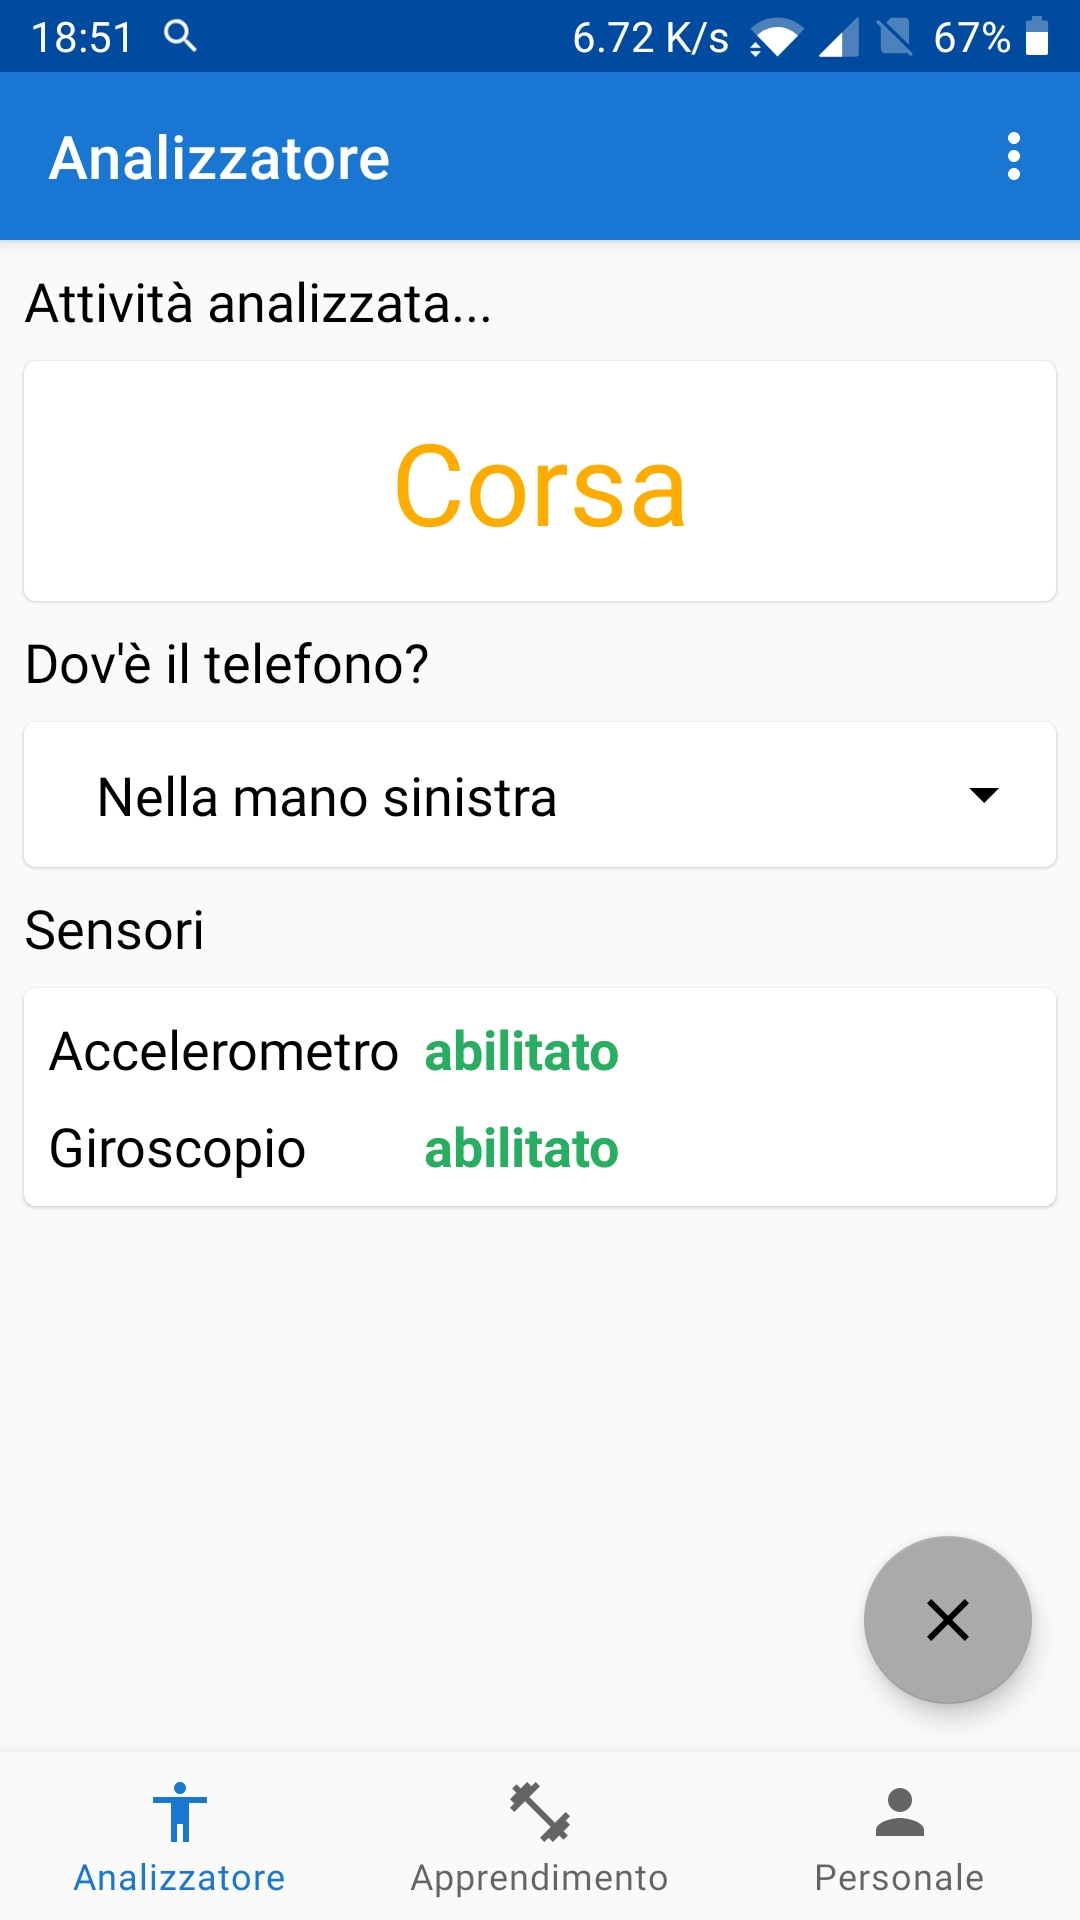
\includegraphics[scale = 0.1019]{assets/images/screenshots/1d_Prediction.jpg}
    \caption{Le 4 fasi dell'analisi}
    \label{fig:screenshots_analysis}
\end{figure}


\subsection{Sezione di apprendimento}
La sezione di apprendimento consente di incrementare l'insieme di informazioni a disposizione del classificatore. 
Si vogliono raccogliere dati inerziali di precise attività su cui, come vedremo nel capitolo \ref{chapter:classification}, la rete neurale si baserà per 
la generazione di modelli sempre più accurati.

\vspace{5mm} %5mm vertical space

Il processo è simile a quanto appena visto. La differenza consiste nel fatto che alle informazioni ottenute dai sensori è 
aggiunta l'attività selezionata manualmente dall'utente.

\vspace{5mm} %5mm vertical space

In questa fase è data piena fiducia all'utilizzatore sulla correttezza dei dati inseriti e sull'attività svolta.

\subsubsection{Fase 1: Inizializzazione}
In una prima fase l'applicazione richiede in autonomia alle API le informazioni di cui necessita. Si cercano:
\begin{itemize}
    \item le informazioni relative alle posizioni del dispositivo selezionabili
    \item la lista di attività addestrabili e il tempo necessario per il loro apprendimento
\end{itemize}
È immediato ottenere tali informazioni mediante richieste ai due endpoints relativi, i cui esempi di risposta sono mostrati nei codici 
\ref{listing:response-activities} e \ref{listing:response-positions}.
Una volta ricevute le risposte l'utente ha la possibilità di selezionare: 
\begin{itemize}
    \item la posizione in cui desidera tenere il dispositivo durante l'esecuzione dell'attività
    \item l'attività che ha intenzione di addestrare
\end{itemize}
In seguito a queste scelte l'apprendimento può essere avviato.

\subsubsection{Fase 2: Preparazione}
Anche in questo frangente sarà inizializzato un servizio in foreground \cite{services} che si occuperà di svolgere 
tutte le azioni necessarie per le fasi seguenti e la UI continuerà ad essere aggiornata con le informazioni ricevute da esso.

Nuovamente, come prima cosa, viene contattato il server per stabilire una connessione TCP. 
In seguito alla ricezione di una risposta affermativa sarà avviato il conto alla rovescia utile come \textit{tempo di preparazione}.

\subsubsection{Fase 3: Apprendimento}
Allo scadere del tempo sono avviati in parallelo un ulteriore countdown e tutti i sensori per la raccolta dei dati.

Il secondo conto alla rovescia indica il \textit{tempo di apprendimento} necessario. I secondi previsti potrebbero differire tra le diverse attività, 
in base alle informazione ottenute nella prima fase. 

Fino allo scadere del tempo tutti i dati raccolti dai sensori sono inviati al \textit{server}, di cui abbiamo precedentemente discusso.

\begin{figure}[H]
    \centering
    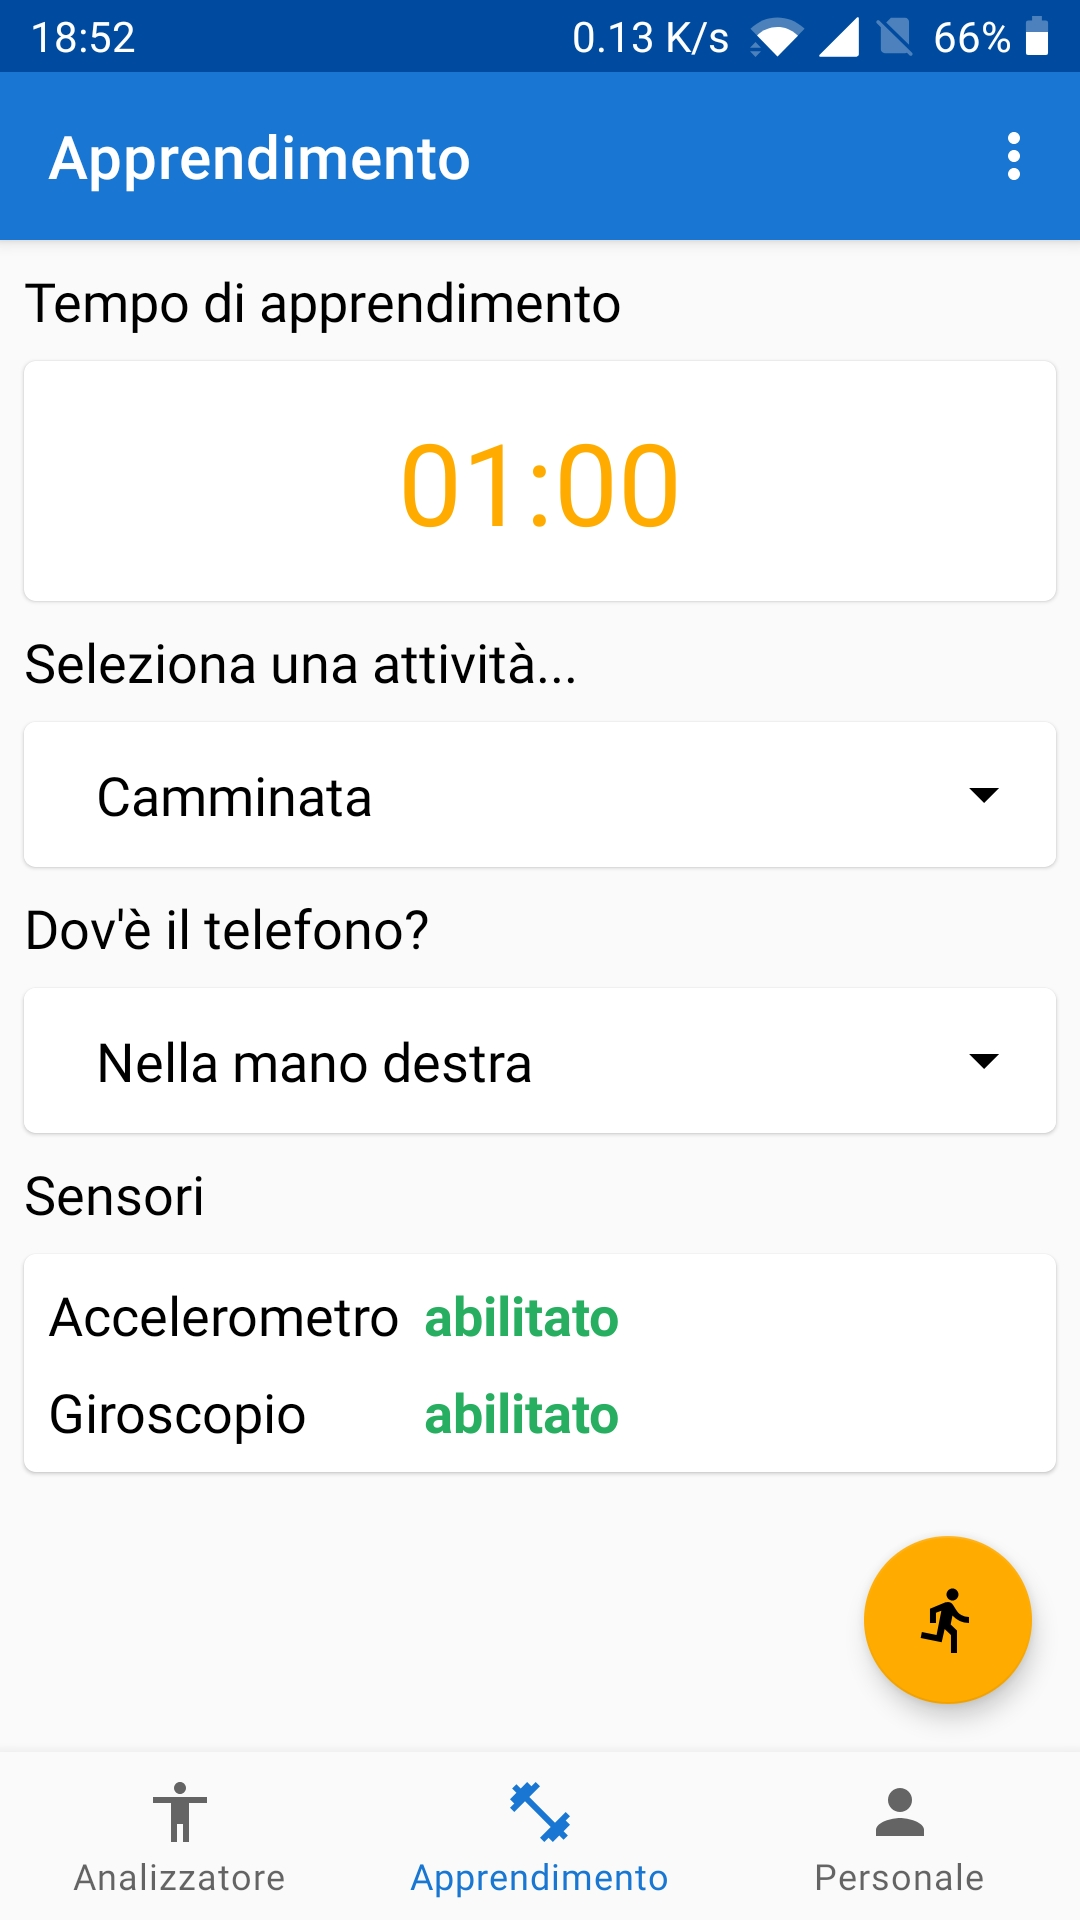
\includegraphics[scale = 0.1019]{assets/images/screenshots/2a_Init.jpg}
    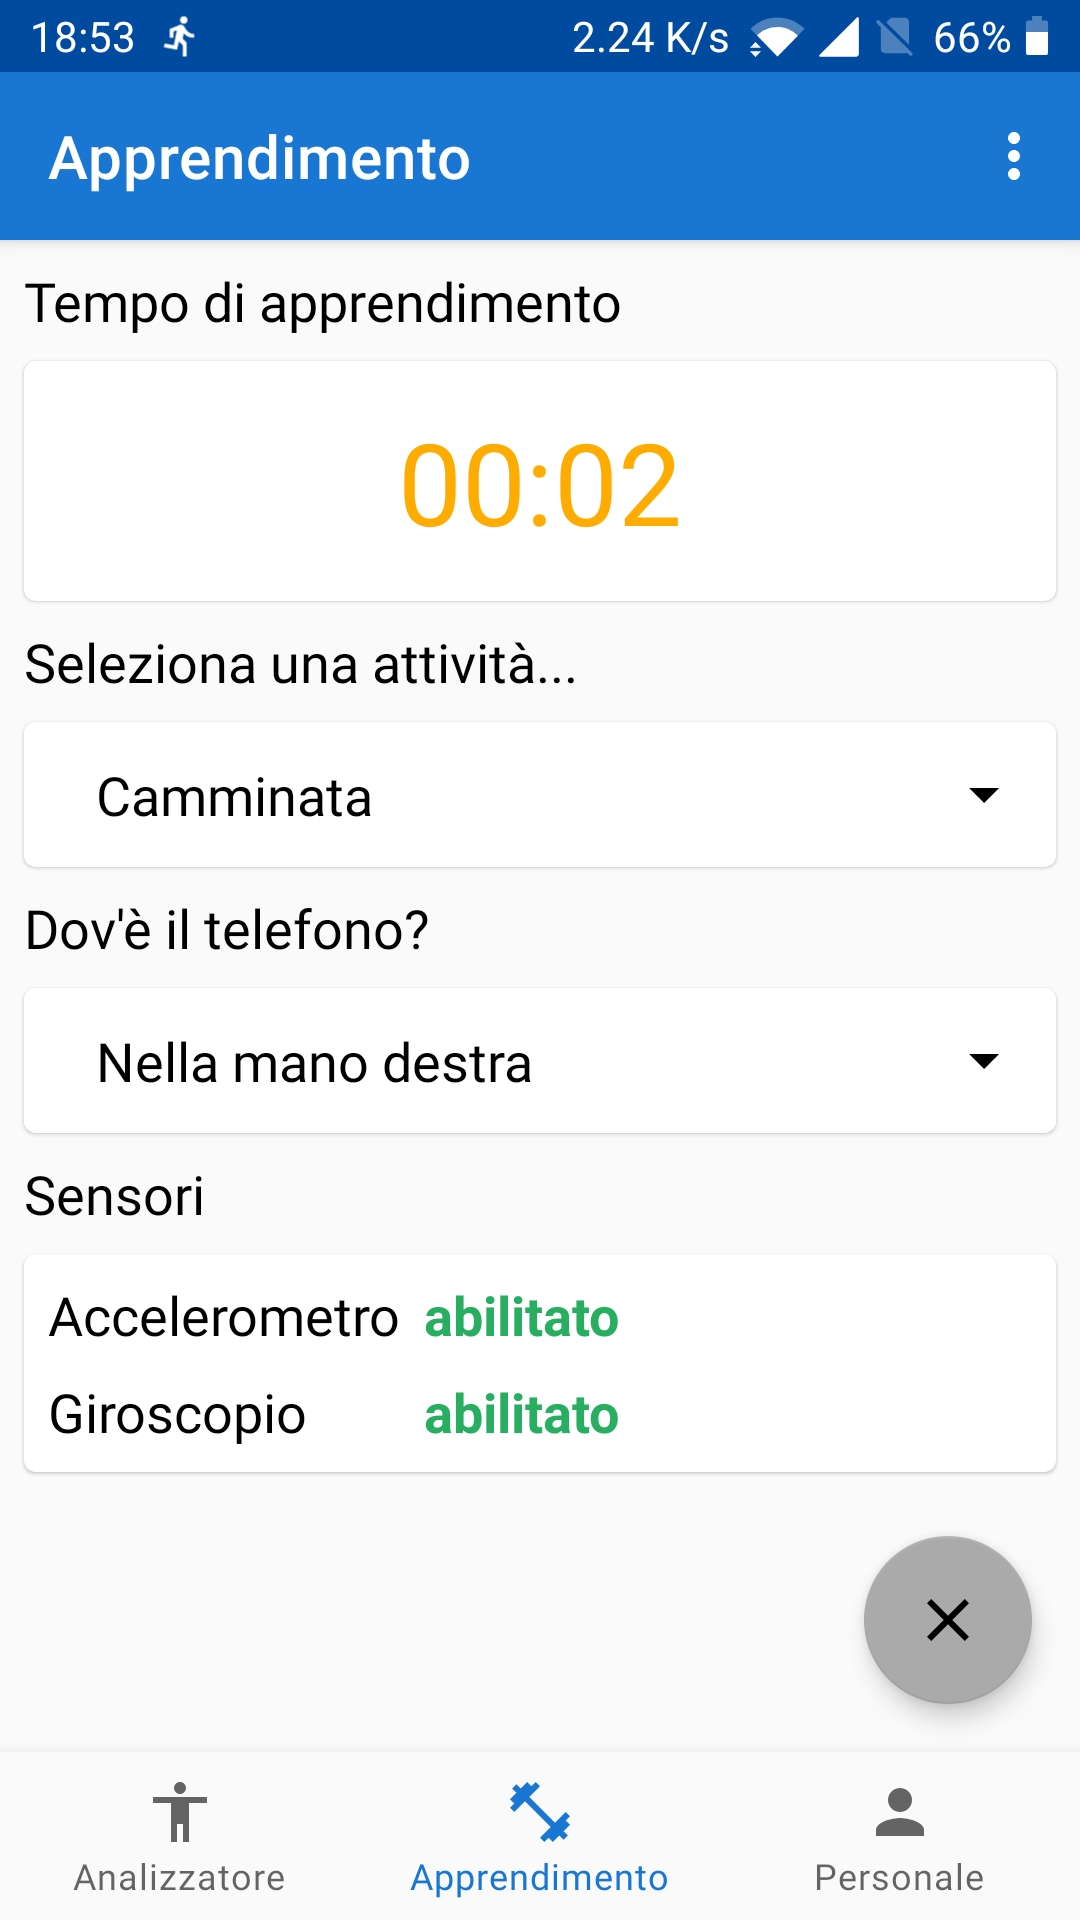
\includegraphics[scale = 0.1019]{assets/images/screenshots/2b_Preparation.jpg}
    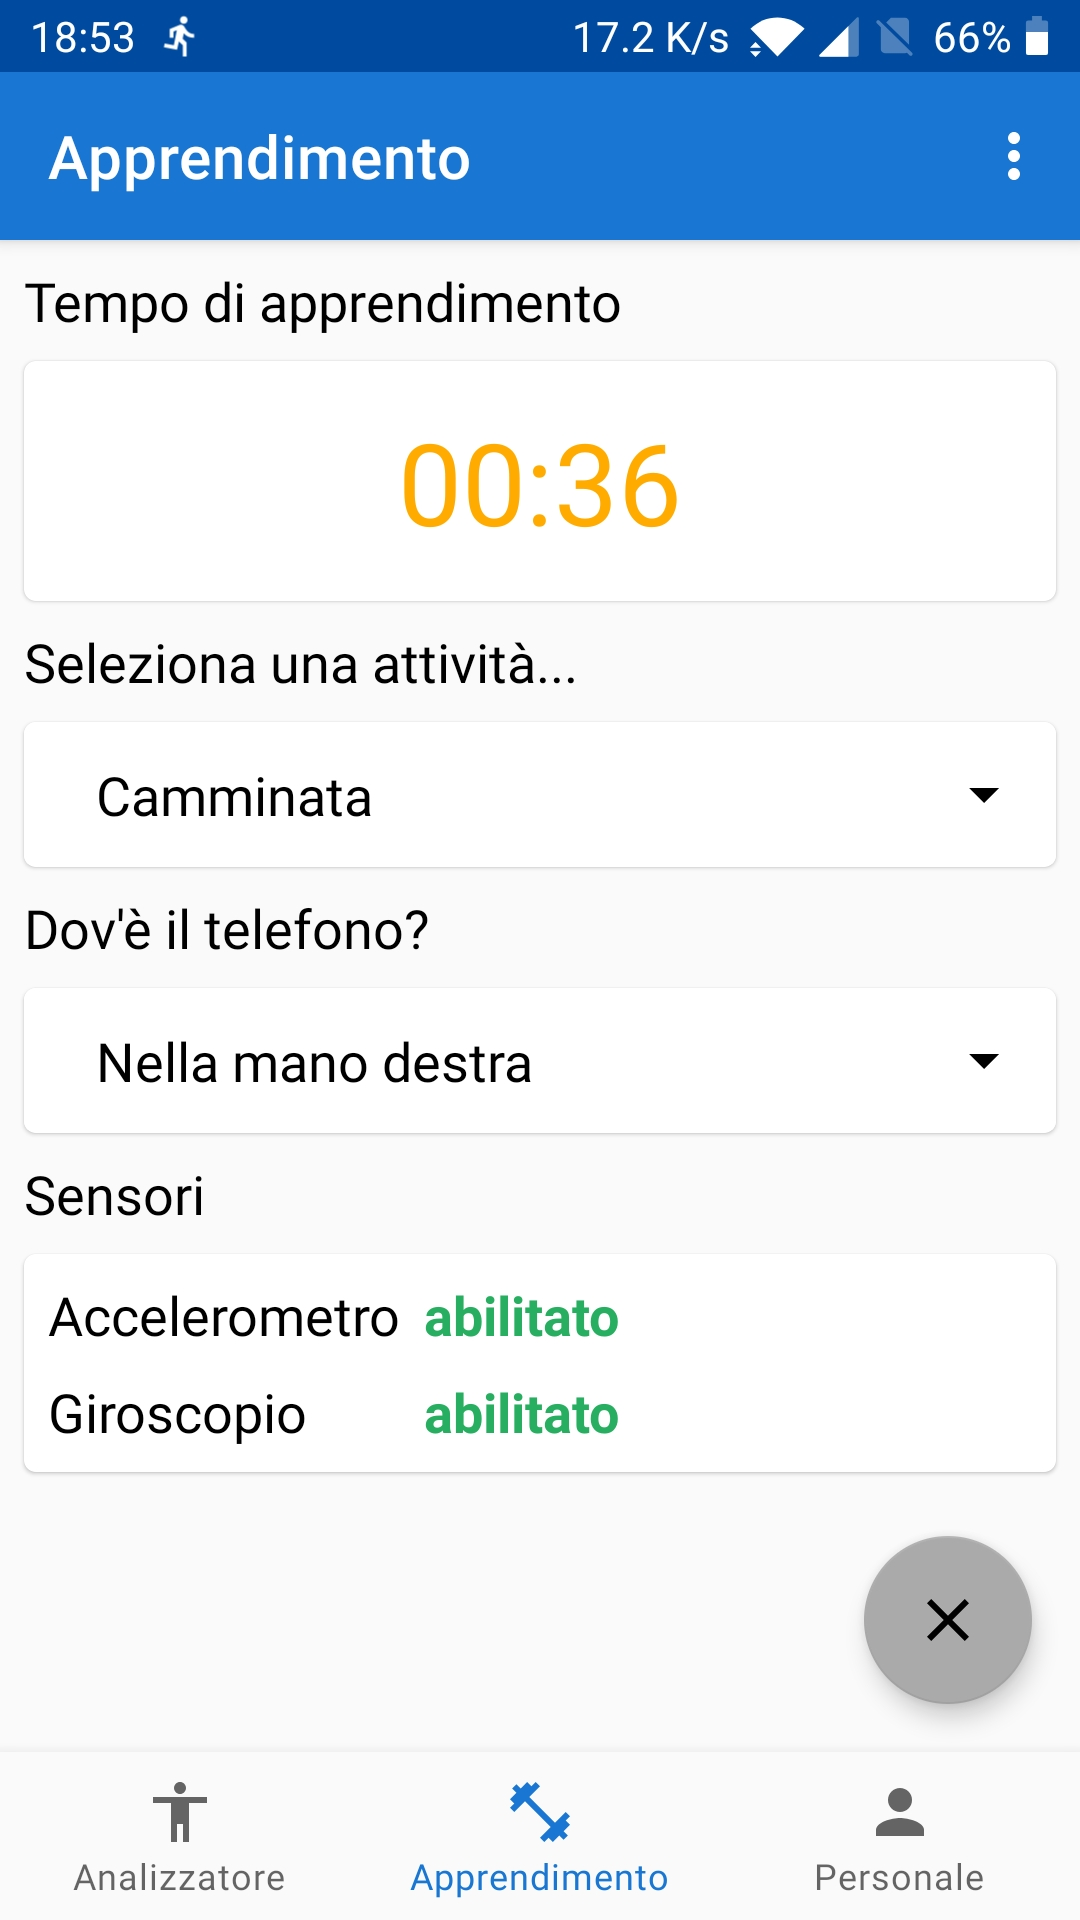
\includegraphics[scale = 0.1019]{assets/images/screenshots/2c_Learning.jpg}
    \caption{Le 3 fasi dell'apprendimento}
    \label{fig:screenshots_learning}
\end{figure}


\subsection{Sezione per l'inserimento di dati aggiuntivi}
La sezione per l'inserimento di dati aggiuntivi permette l'aggiunta di ulteriori informazioni 
che potrebbero tornare utili durante il riconoscimento dell'attività.
Un esempio pratico potrebbe essere l'utilizzo di informazioni riguardanti i dati fisici dell'utente (altezza, peso, etc.) qualora 
si ritenesse rilevante il loro valore per la classificazione.

\begin{figure}[H]
    \centering
    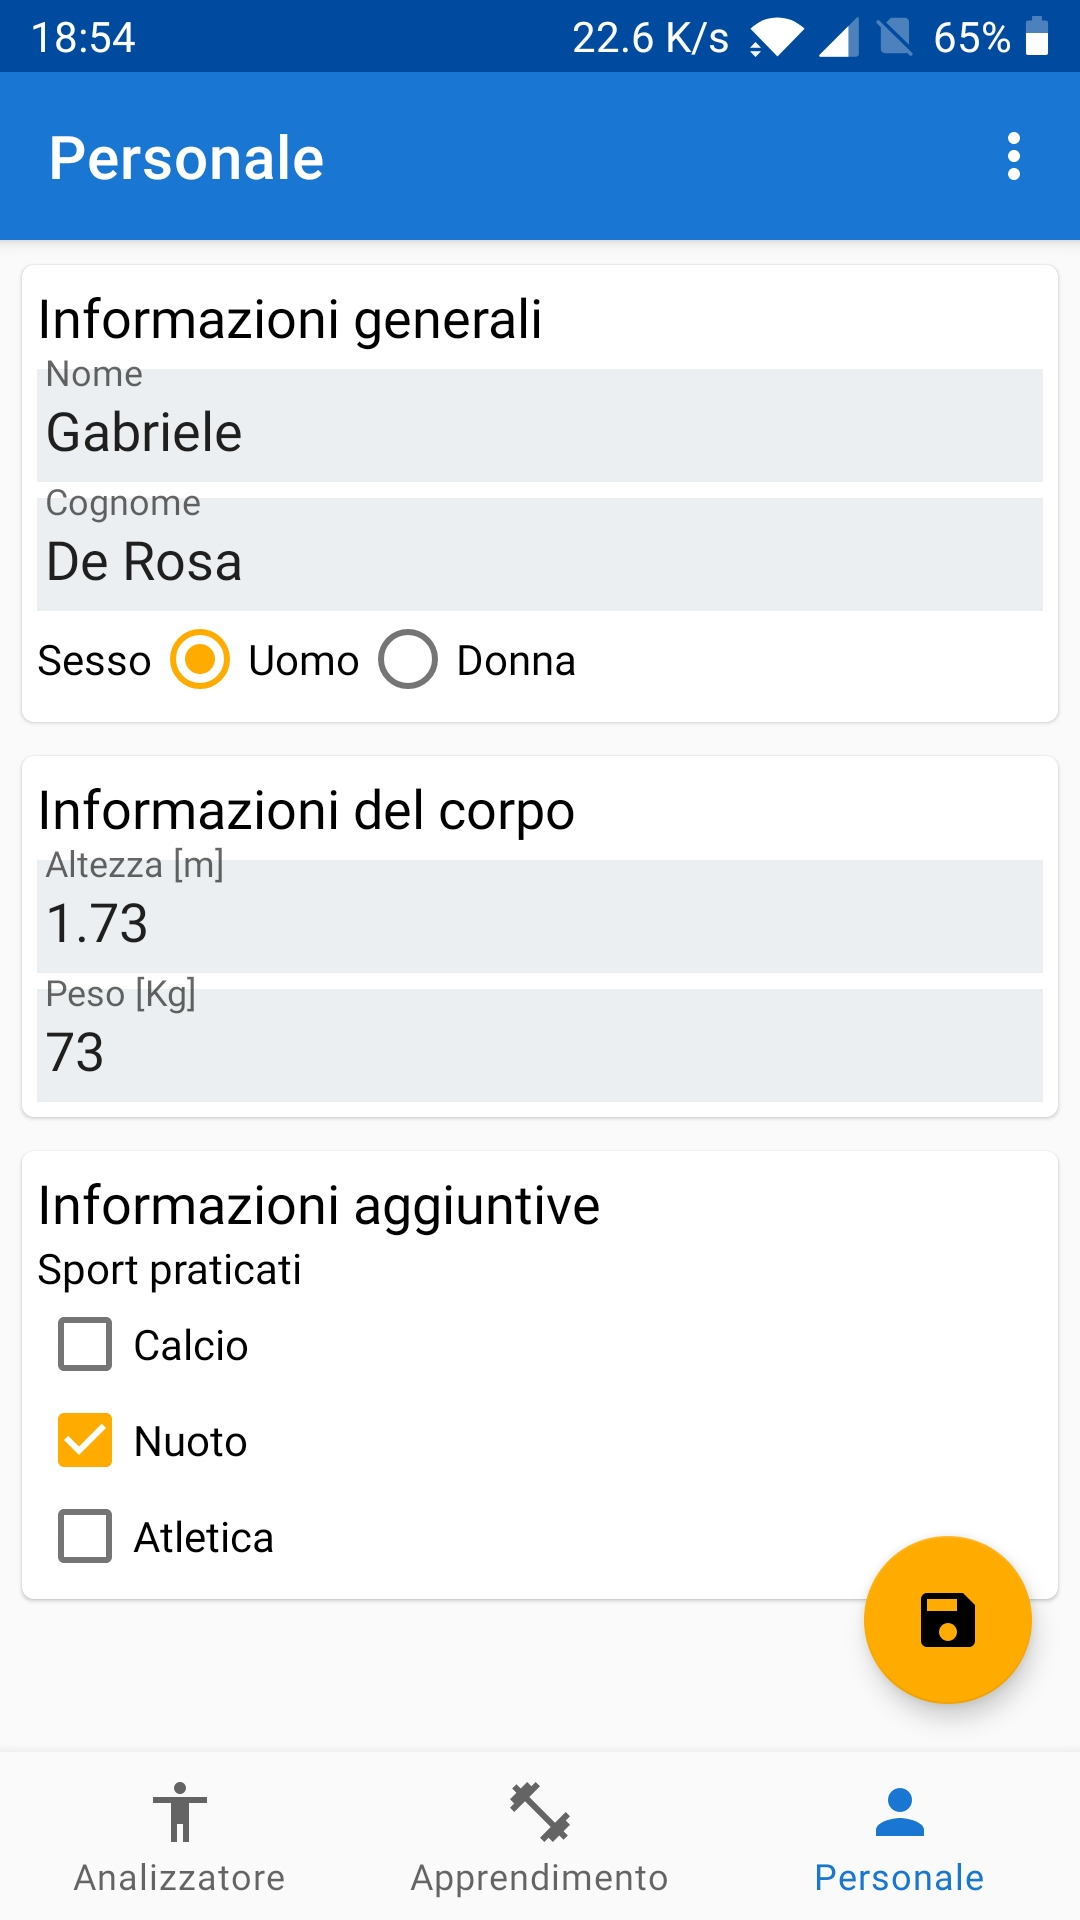
\includegraphics[scale = 0.1019]{assets/images/screenshots/3a_Init.jpg}    
    \caption{Il modulo di inserimento dati generato programmaticamente}
    \label{fig:screenshots_personal}
\end{figure}

\subsubsection{Generazione del layout}
Ritengo opportuno soffermarmi maggiormente sulla generazione del layout di questa sezione.

\vspace{5mm} %5mm vertical space

Malgrado agli occhi dell'utilizzatore appaia come un semplice modulo di inserimento dati, 
la generazione di ogni componente dello stesso avviene in modo dinamico.
L'intero modulo è generato programmaticamente a partire dalle informazioni ricevute in risposta da una richiesta al relativo endpoint delle API. 

Questa opportunità permette ad un amministratore di sistema di variare le informazioni richieste
senza dover rilasciare un aggiornamento dell'applicazione.

\vspace{5mm} %5mm vertical space

Per facilitarne la comprensione è possibile vederne l'applicazione in un esempio. La risposta di esempio mostrata nel codice 
\ref{listing:response-form} è in grado di generare il layout di figura \ref{fig:screenshot_layout_from_code}.

\begin{figure}[H]
    \centering
    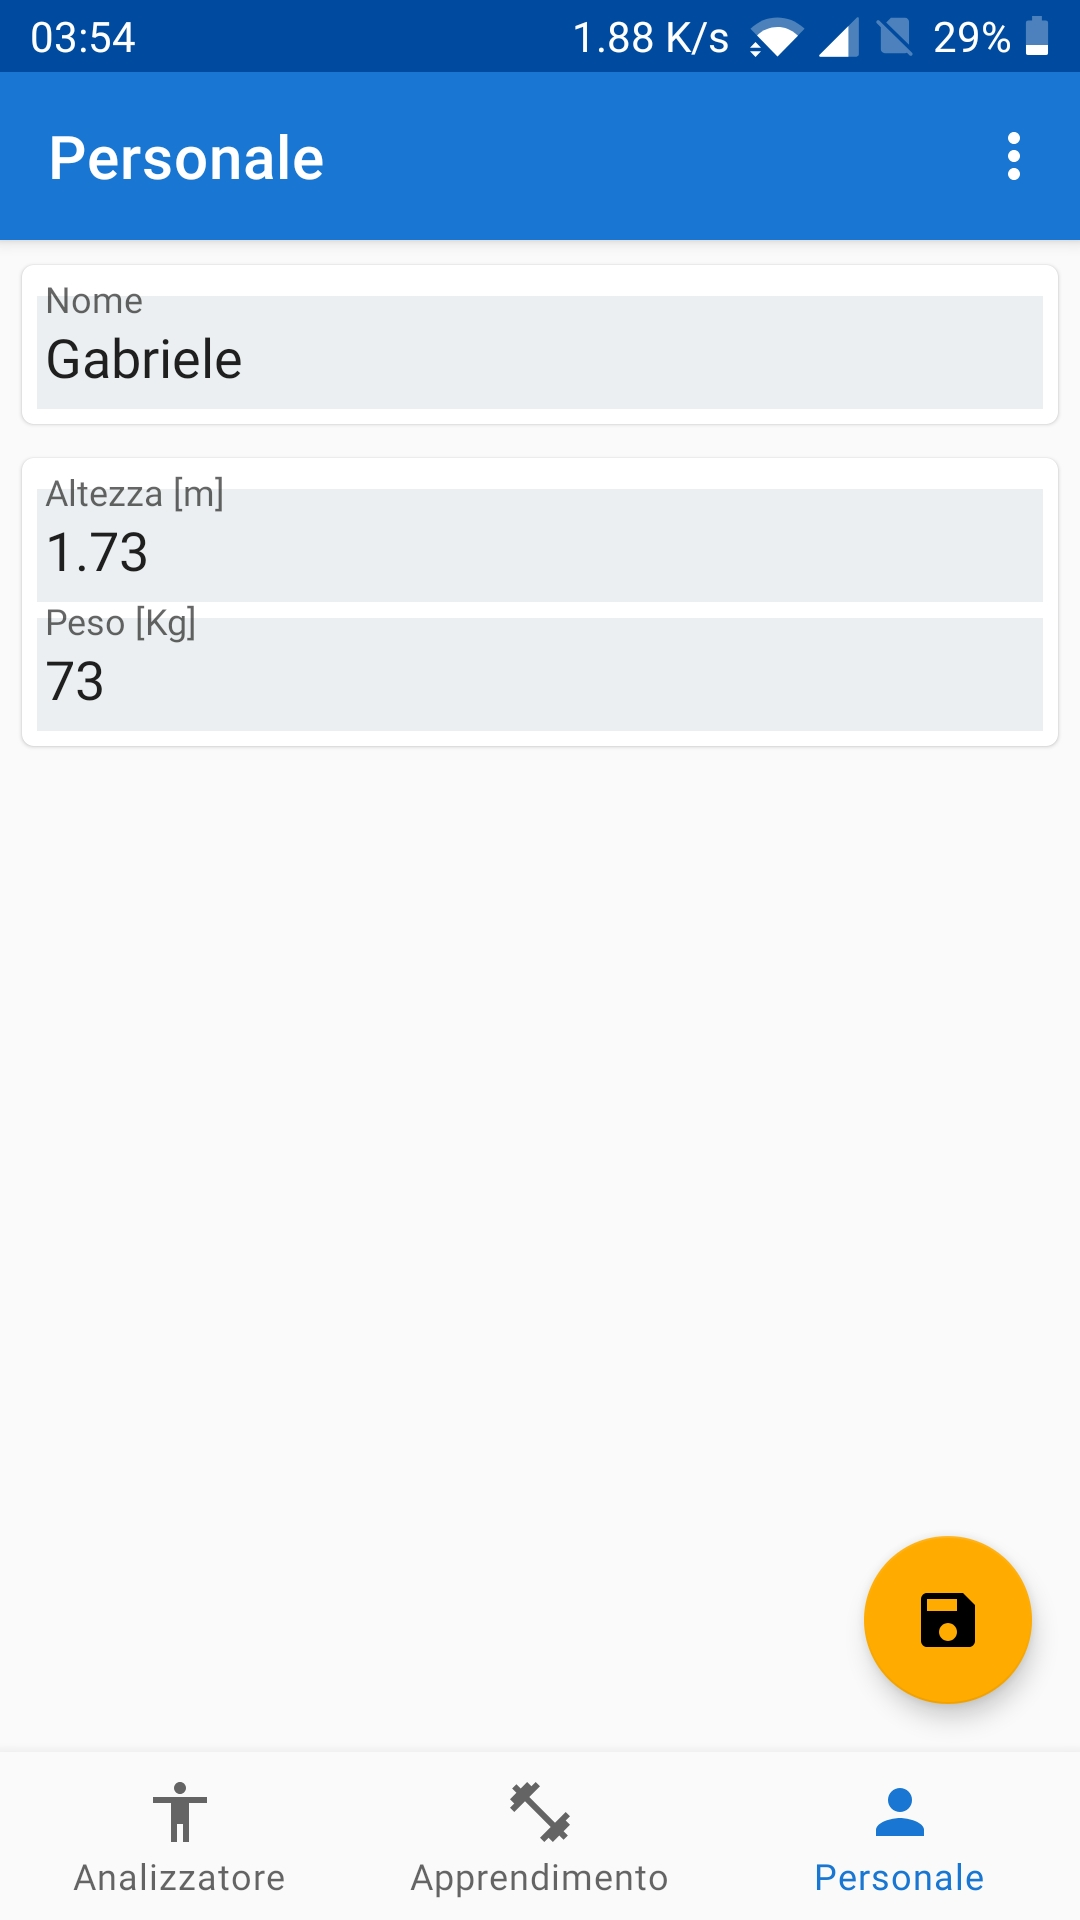
\includegraphics[scale = 0.1019]{assets/images/screenshots/3b_Layout_from_code.jpg}    
    \caption{Esempio di modulo generato dalle informazioni del codice \ref{listing:response-form}}
    \label{fig:screenshot_layout_from_code}
\end{figure}


\newpage
\section{Feedback sonoro}
Dal funzionamento che abbiamo appena visto è intuibile che l'app possa essere utilizzata con il dispositivo situato in posizioni che non permetterebbero
un collegamento visivo diretto. Ad esempio, quando la posizione selezionata è \textit{nelle tasche}.

Tale situazione renderebbe impossibile l'accesso alle informazioni relative al progresso dell'attività in corso, che sia 
un'analisi o un apprendimento.
Questa eventualità ha reso necessaria l'implementazione di un feedback sonoro realizzato mediante le librerie 
di sintetizzazione vocale per il \textit{text to speech} \cite{tts} offerte da Android.

Oltre al feedback visivo è offerto quindi un feedback sonoro per tutte le informazioni rilevanti, come l'inizio e la fine dell'attività, 
il conto alla rovescia ed i risultati dell'attività ipotizzata.

\vfill
\begin{listing}[H] 
    \inputminted[frame=single,framesep=10pt]{java}{assets/snippets/app/voice.java}
    \caption{Implementazione del text to speech in Android}
\end{listing}



\section{Countdown Timers}
I countdown che regolano il tempo di svolgimento delle attività sono implementati utilizzando la 
classe \textit{CountDownTimer} \cite{countdown} offerta direttamente da Android.
\begin{listing}[H] 
    \inputminted[frame=single,framesep=10pt]{java}{assets/snippets/app/countdown.java}
    \caption{Implementazione di un conto alla rovescia}
\end{listing}
\noindent Entrambi i timer implementati (\textit{timer di preparazione} e \textit{timer di apprendimento}) non hanno un tempo stabilito in partenza. 

Il tempo utile per la preparazione è settabile dall'utente tra le impostazioni dell'applicazione, invece il tempo di 
apprendimento è ottenuto tramite la relativa richiesta alle API e può dipendere dall'attività selezionata.



\section{Accesso alle API}
Le richieste agli endpoints, di cui abbiamo discusso le varie applicazioni per l'ottenimento delle informazioni preliminari, 
sono fatte utilizzando la libreria Retrofit. 

Implementando delle classi Java che modellano la struttura delle risposte dell'API si riescono ad ottenere facilmente 
tutte le informazioni richieste.

\subsubsection{Retrofit}
Retrofit \cite{retrofit} è una libreria open source nata per trasformare una richiesta ad una RESTful API 
in una \textit{Java Interface}.


\newpage
\section{Sensori di movimento}
I sensori di movimento utilizzati sono \textbf{accelerometro} e \textbf{giroscopio}.

Entrambi presentano gli stessi valori informativi (i tre assi x, y, z), pertanto durante lo sviluppo sono stati gestiti in modo analogo.

\subsection{Attivazione dei sensori}
I sensori del dispositivo sono gestiti direttamente dal sistema operativo. Pertanto Android rende disponibile 
un gestore (\textit{SensorManager} \cite{sensor_manager}) per richiederne l'attivazione e la disattivazione.

\begin{listing}[H] 
    \inputminted[frame=single,framesep=10pt]{java}{assets/snippets/app/sensors/start_sensors.java}
    \caption{Attivazione dei sensori}
    \label{listing:sensor-activation}
\end{listing}
\begin{listing}[H] 
    \inputminted[frame=single,framesep=10pt]{java}{assets/snippets/app/sensors/stop_sensors.java}
    \caption{Disattivazione dei sensori}
    \label{listing:sensor-deactivation}
\end{listing}

\vfill
\subsubsection{Frequenza di campionamento}
\label{paragraph:sampling_rate}
Ho scelto una frequenza di campionamento di $20$ Hz, che corrisponde ad avere una acquisizione 
ogni 
$$T_c = \frac{1}{20} = 0.5 s = 50ms $$

\vspace{5mm} %5mm vertical space
\noindent Si può notare come $50ms$ sia proprio il periodo di campionamento impostato 
all'attivazione dei sensori nel codice \ref{listing:sensor-activation}.


\newpage
\subsection{Estrazione dei dati inerziali}
Dopo l'attivazione dei sensori il sistema operativo richiama una specifica funzione di \textit{callback} ogni volta 
che si realizza un evento, ovvero ad ogni nuova acquisizione.

È quindi necessario implementare l'interfaccia \textit{SensorEventListener} \cite{sensor_listener} definendo la 
callback con l'opportuna gestione dei dati inerziali ottenuti.

\subsubsection{Callback}
Una callback è una specifica funzione richiamata dal sistema operativo al verificarsi di un determinato evento.
Il suo scopo è quello di consentire l'implementazione di una gestione personalizzata dell'evento che l'ha invocata.
\vfill
\begin{listing}[H] 
    \inputminted[frame=single,framesep=10pt]{java}{assets/snippets/app/sensors.java}
    \caption{Implementazione della callback per gli eventi dei sensori}
    \label{listing:sensor-event-callback}
\end{listing}

\newpage
\section{Comunicazioni con il server}
Oltre a ricavare le informazioni dai sensori è ovviamente necessario procedere al loro invio al server  
dove verranno processate come visto nella sezione \ref{section:receiver}.
\subsubsection{Connessione al server}
Per prima cosa è indispensabile avere una connessione attiva. Tale connessione è richiesta all'avvio dei servizi di 
analisi e apprendimento.

Come abbiamo precedentemente discusso si è scelta una connessione TCP via socket. La corrispondente implementazione Java
avviene mediante la classe \textit{Socket} \cite{socket}.
\begin{listing}[H] 
    \begin{minted}[frame=single,framesep=10pt]{java}
socket = new Socket(DESTINATION, PORT);
    \end{minted}
    \caption{Implementazione della connessione via socket}
\end{listing}

\subsubsection{Invio di un messaggio}
Una volta attivata la connessione si può procedere all'invio dei dati ogni qual volta il sistema 
operativo notifica un cambiamento di stato dei sensori. All'interno della callback implementata, vista in precedenza, è
richiamato il metodo per l'invio dei messaggi.
\begin{listing}[H] 
    \inputminted[frame=single,framesep=10pt]{java}{assets/snippets/app/connection/send.java}
    \caption{Implementazione dell'invio di un messaggio}
\end{listing}

\newpage
\subsubsection{Ricezione di un messaggio}
La ricezione delle risposte da parte del server avviene invece banalmente rimanendo in ascolto 
dei messaggi in arrivo.
\begin{listing}[H] 
    \inputminted[frame=single,framesep=10pt]{java}{assets/snippets/app/connection/receive.java}
    \caption{Implementazione della ricezione di un messaggio}
\end{listing}
\vspace{5mm} %5mm vertical space
\noindent Ogni messaggio ricevuto viene elaborato in base alla tipologia. Alcuni di essi rappresentano solo una conferma di avvenuta 
connessione o di corretta ricezione dei messaggi inviati, mentre altri contengono informazioni da mostrare direttamente all'utente.

\vspace{5mm} %5mm vertical space
In precedenza, nel codice \ref{listing:example-message-prediction}, abbiamo visto uno dei messaggi inviati dal \textit{modulo di comunicazione} come risposta. 
Tutti i messaggi di questo genere sono ricevuti dall'applicazione in questa fase.